
\chapter{Конструкторская часть}\label{Konstruct}
%\addcontentsline{toc}{chapter}{2 Конструкторская часть}

В данном разделе представлены схемы алгоритмов. Так же будут описаны пользовательские структуры данных, 
приведены классы эквивалентности для тестирования реализуемого ПО.

\section{Схемы}\label{SchemaAlg}

На рисунке \ref{ris:schemaposav} показана траектория заявки.

\begin{figure}[H]
  \center{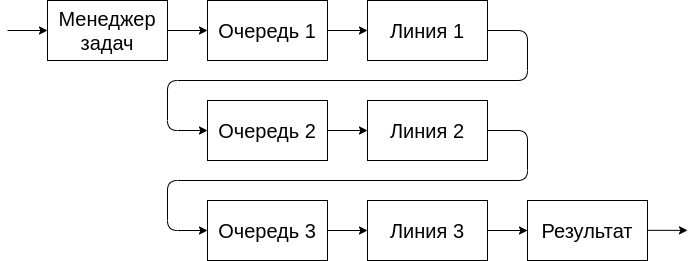
\includegraphics[scale=0.60]{l1.route}}
  \caption{Траектория заявки}
  \label{ris:schemaposav}
\end{figure}

На рисунке \ref{ris:schemaparrowav} показан принцип работы конвейера. После того, как первая заявка будет обработана на первом этапе,
она поступит на второй, а на первый этап придет 2 заявка, таким образом две линии будут работать параллельно. Когда первая заявка 
будет обработана на 2 этапе, она попадет в 3 линию конвеера. Как толко первая линия обработает 2 заявку, она получит третью заявку.

\begin{figure}[H]
  \center{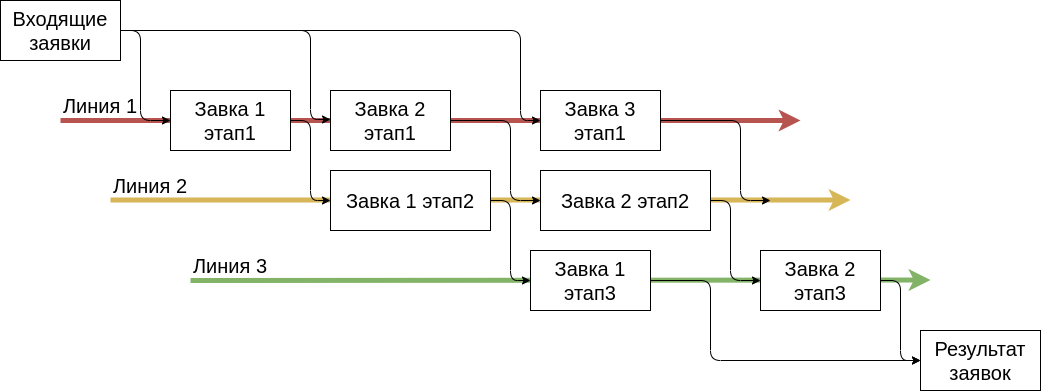
\includegraphics[scale=0.45]{l1.idea}}
  \caption{Принцип работы конвеера}
  \label{ris:schemaparrowav}
\end{figure}


\section{Структуры данных}\label{Structs}

При реализации приведенных алгоритмов потребуется тип данных: заявка.
Она должна содержать следующие поля:

\begin{itemize}
  \item строка, поступившая на вход,
  \item строка - результ,
  \item время поступления в конвейер,
  \item массив времени этапов (время этапов содержит время начала обработки и конца).
\end{itemize}

\section{Тестирование}\label{Testing}

Для алгоритма шифрования строк можно выделить следующие классы эквивалентности:

\textit{Шифр Цезаря}

\begin{enumerate}
    \item символы, где i+key<n, 
    \item символы, где i+key>n.
\end{enumerate}

\textit{Шифр Атбаш}

\begin{enumerate}
    \item символы, где i<n/2, 
    \item символы, где i>n/2.
\end{enumerate}

\textit{Шифр XOR}

\begin{enumerate}
    \item символы, где i xor key < n, 
    \item символы, где i xor key > n.
\end{enumerate}

%\subsection{Способы тестирования}\label{TestingMethods}

%При разработке программы удобно использовать следующие методы тестирования:

%\begin{enumerate}
%    \item Модульные тесты 
%    \item Функциональные тесты 
%\end{enumerate}

\section{Вывод конструкторской части}\label{KonstructResult}
На основе данных, полученных в аналитическом разделе, были построены схемы конвеерной обработки,
выделены необходимые для реализации структуры данных и методы тестирования.

